\documentclass{article}

\makeatletter
\newif\ifhtlatex
\@ifpackageloaded{tex4ht}{\htlatextrue}{\htlatexfalse}
\makeatother

\usepackage{amsmath}
\usepackage[margin=0.93in]{geometry}
\usepackage{graphicx}
\usepackage{calc}

\usepackage{hyperref}
\hypersetup{colorlinks=true,allcolors=[rgb]{1,0.56,0}}

\def\name{Peter B.~Denton, Ph.D.}
\title{CV}

\pagestyle{myheadings}
\markright{\name}
\thispagestyle{empty}

\usepackage{sectsty}
\sectionfont{\rmfamily\mdseries\Large}
\subsectionfont{\rmfamily\mdseries\bfseries\large}
\subsubsectionfont{\rmfamily\mdseries\itshape\normalsize}

\setlength\parindent{0em}

\renewenvironment{itemize}{
\begin{list}{}{
\setlength{\leftmargin}{.5em}}}{
\end{list}}

\begin{document}

\ifhtlatex
\Tag{TITLE+}{CV}
\fi

% % % % % With headshot
% 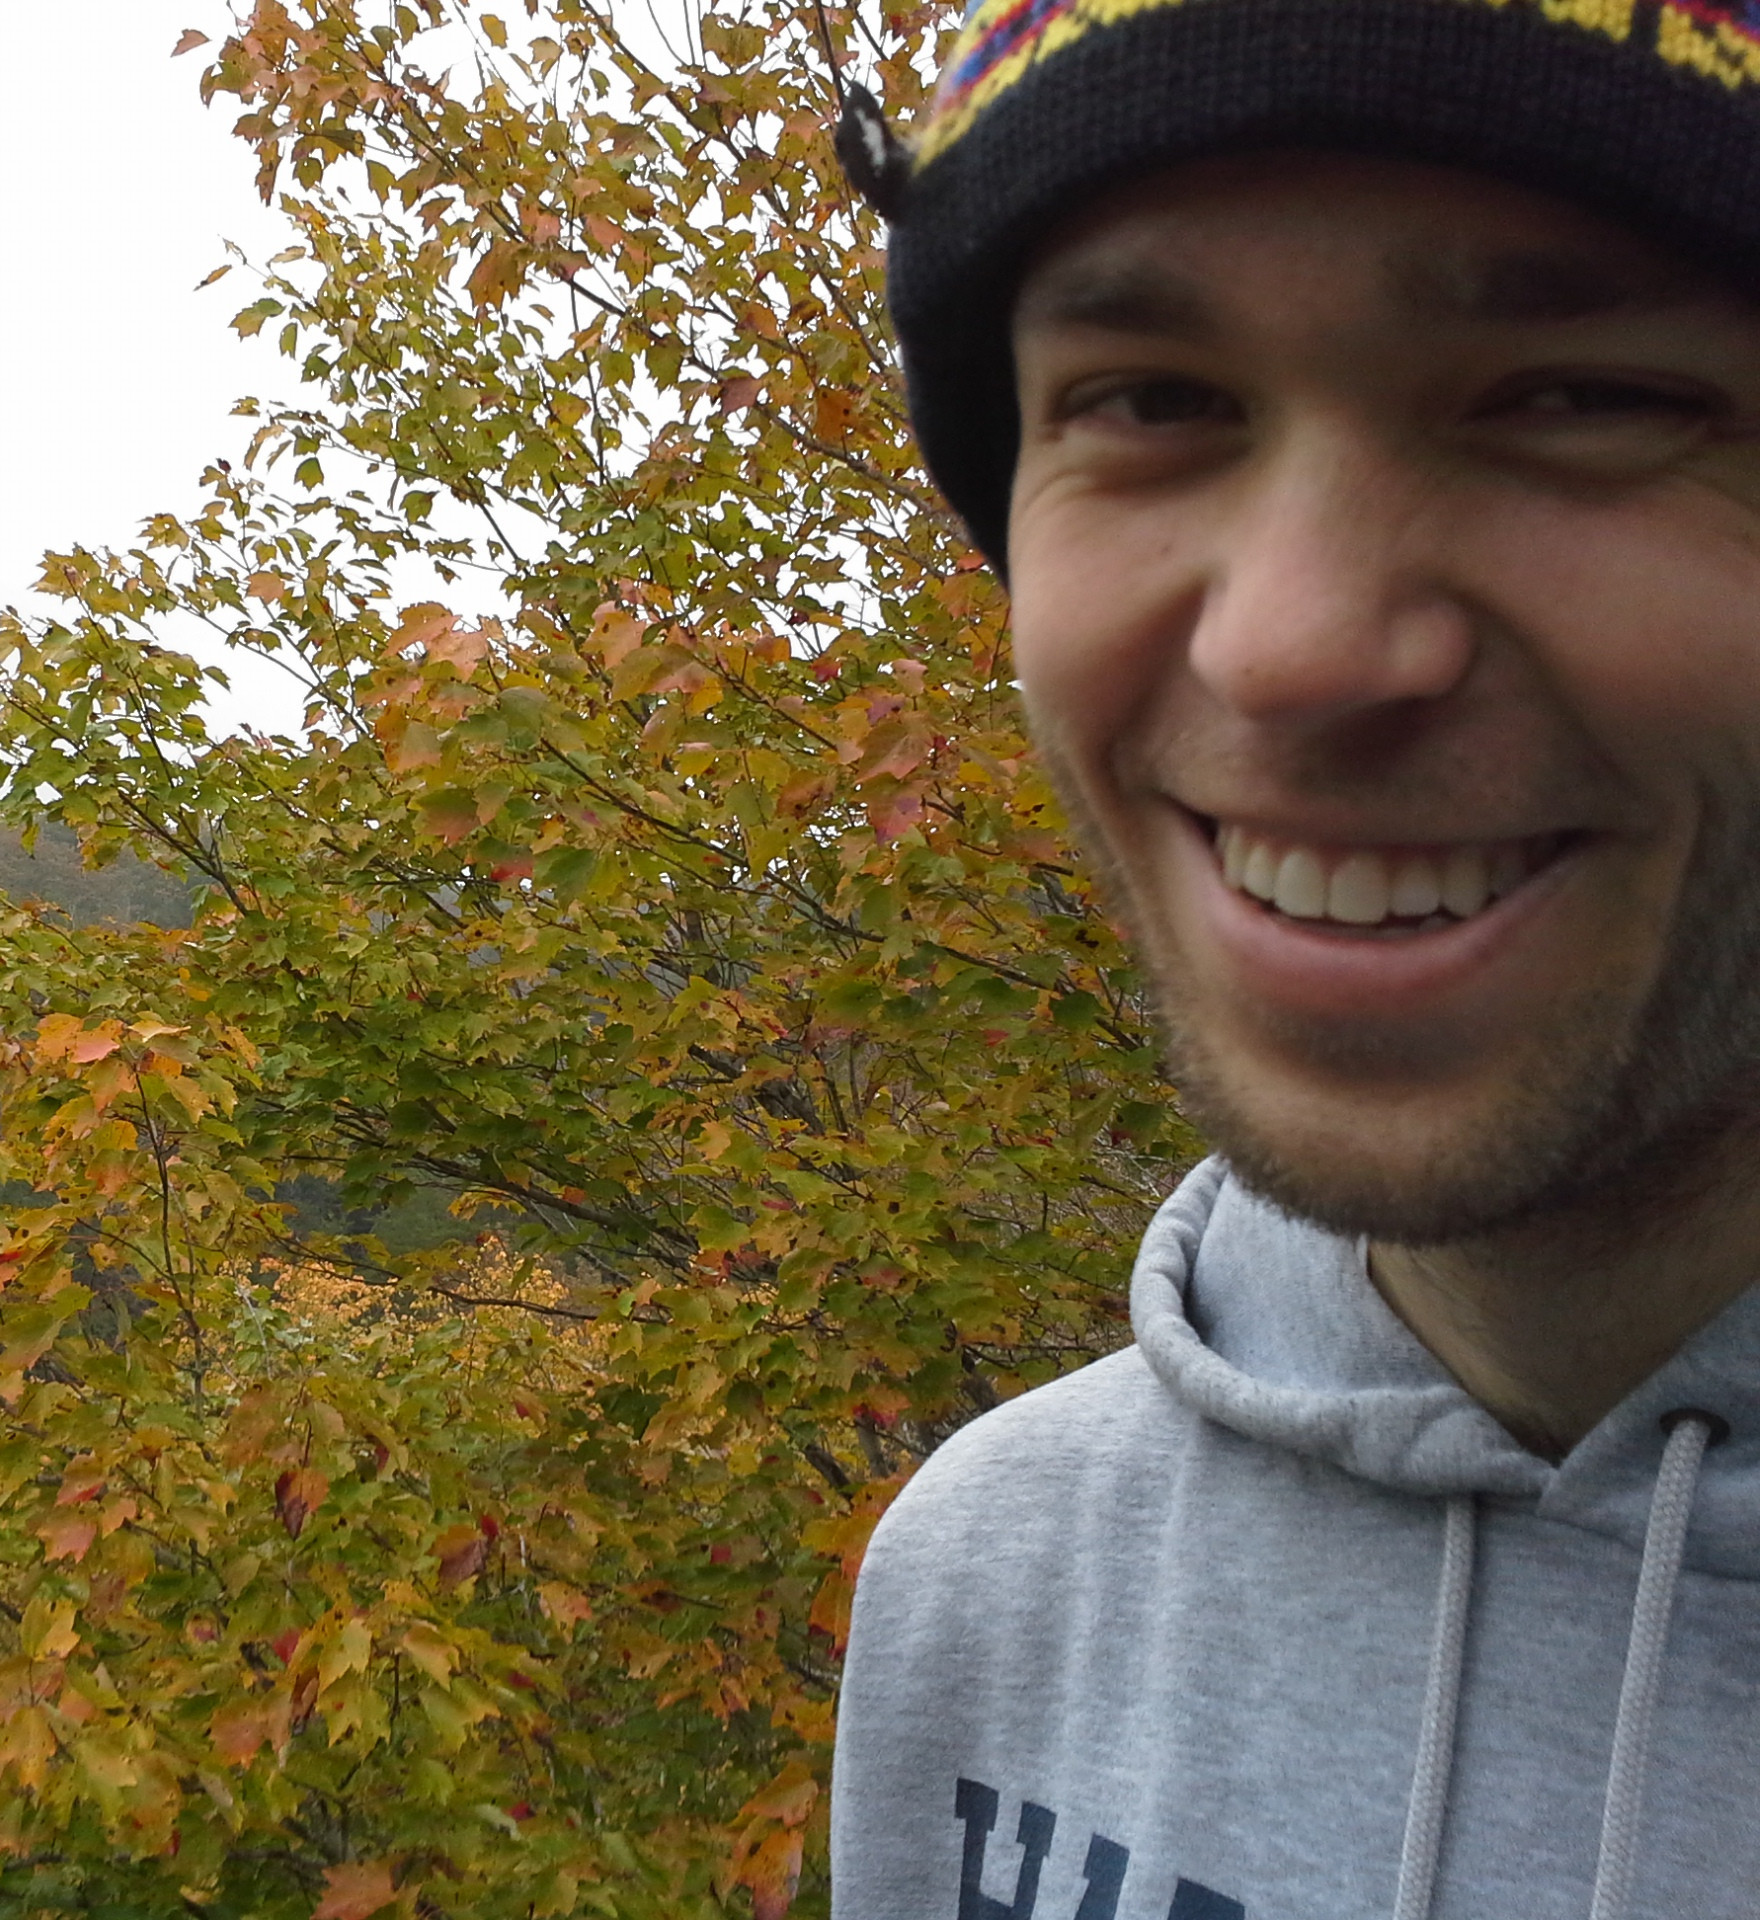
\includegraphics[width=1.2in]{face_cropped}
% \parbox{\textwidth-1.3in}{\vspace*{-1.1in}
% {\huge \name}\\
% \vspace*{0.1in}
% \begin{tabular}{ll|l|ll}
% +45 71 49 29 40 & Gernersgade 35, 1 th & Updated: & \today\\
% \href{mailto:peterbd1@gmail.com}{\tt peterbd1@gmail.com} & Copenhagen K 1319 & Website: & 
% \href{http://peterdenton.github.io}{\tt peterdenton.github.io}
% \end{tabular}
% }

% % % % % Without headshot
\vspace*{-0.5in}
{\huge \name}\hfill\includegraphics[height=0.4in]{BNL}\\
\vspace{0.1in}
\begin{tabular}{ll|l|ll}
Phone: & +1-631-344-3767 & Bldg 510A PO Box 5000 & Updated: & \today\\
Email: & \href{mailto:peterbd1@gmail.com}{\tt peterbd1@gmail.com} & Upton, NY 11973 & Website: & 
\href{http://peterdenton.github.io}{\tt peterdenton.github.io}
\end{tabular}

\subsection*{Research Experience}
\begin{itemize}
\item Physicist at Brookhaven National Laboratory, January 2024--Present.
\item Associate Physicist at Brookhaven National Laboratory, October 2020--December 2023.
\item Assistant Physicist at Brookhaven National Laboratory, October 2018--September 2020.
\item Postdoctoral Fellow with Irene Tamborra at Niels Bohr International Academy, September 2016--August 2018.
\item Graduate Student Research Program in Theoretical Physics with Stephen Parke at Fermilab, August 2015--August 2016.
\item DOE funded research assistant with Thomas J.~Weiler at Vanderbilt University, Spring 2011--Fall 2015.
\item Research assistant with Sokrates Pantelides at Vanderbilt University, Summer--Fall 2010.
\item Lee Teng Internship with Tanaji Sen at Fermilab, Summer 2009.
\item Bonner Labs with Bill Llope at Rice University, Summer 2008.
\end{itemize}

\subsection*{Research Interests}
\begin{itemize}
\item SM and BSM neutrino theory.
\item Astroparticle physics.
\item Black hole phenomenology.
\item Dark matter physics.
\end{itemize}
Published papers \href{https://inspirehep.net/authors/1272961}{[inspire]}, \href{https://arxiv.org/search/?searchtype=author&query=Denton\%2C+P+B}{[arXiv]}

\subsection*{Degrees}
\begin{itemize}
\item Ph.D.~Physics, Vanderbilt University, August 2016.
\item B.S.~Physics, Rice University, May 2010.
\item B.A.~Mathematics, Rice University, May 2010.
% \item Multi-variable calculus, differential equations, Grand Rapids Community College, 2005--2006.
\end{itemize}

\subsection*{Honors and Awards}
\begin{itemize}
\item Physical Review D Reviewer Excellence 2024 Award, awarded April 2024.
\item Neutrino Physics Center (NPC) award of to work with Stephen Parke at Fermilab, awarded May 2023.
\item Nominated and selected as the BNL delegate to the 2022 Science and Technology in Society Forum in Kyoto, October 2022.
\item BNL NPP DEI grant \$10,000 to support Apurva Goel, awarded April 2022.
\item Neutrino Physics Center (NPC) award of \$10,000 to work with Stephen Parke at Fermilab, awarded December 2018.
\item Neutrino Theory Network (NTN) award of \$14,000 to work with Irina Mocioiu at PSU, awarded June 2018.
\item The Giorgio Salvini diploma from the Erice International School of Subnuclear Physics, awarded June 2016.
\item PITT PACC travel award to attend Pheno '16, awarded April 2016.
\item Vanderbilt Dissertation Enhancement Grant of \$2,000 to attend the Theoretical Advanced Study Institute, awarded April 2014.
\item Subsidy of \$1,600 to attend the Theoretical Advanced Study Institute: Amplitudes For Colliders in June 2014, awarded April 2014.
\item Division of Particles \& Fields travel grant to the APS April 2013 meeting, awarded March 2013.
\item The Robert T.~Lagemann Award of \$1,000 for highest academic achievement by a first-year graduate student, awarded April 2011.
\item McMinn Fellowship at Vanderbilt of \$25,000 over five years, awarded March 2010.
\end{itemize}

\subsection*{Collaborations}
\begin{itemize}
\item Giant Radio Array for Neutrino Detection (GRAND), 2017--Present.
\item Forward Search Experiment at the LHC (FASER), 2018--Present.
\item Deep Underground Neutrino Experiment (DUNE), 2021--Present.
\item LSST-DESC, 2024--Present.
\end{itemize}

\subsection*{Service}
\begin{itemize}
\item Pub Talk as a part of SURF's Neutrino Day program, July, 2024.
\item Member of BNL's Nuclear and Particle Physics DEI council, 2023--Present.
\item Diversity Professional Leadership mentor through Stony Brook, 2022--Present.
\item Co-chair of Brookhaven Forum 2021 and 2023.
\item Co-chair of NuTau2021.
\item Brookhaven Women In Science (BWIS) member, 2020--Present.
\item Snowmass neutrino oscillations subtopic convener and neutrino theory liaison 2020--2022 organizing many workshops.
\item Interact with grade-school students via APS's \emph{Adopt-A-Physicist}, Skype-A-Scientist, $\dots$ programs, 2018--2021.
\item International Organizing Committee for Neutrino 2020.
\item Convener for Brookhaven Forum 2019, DPF 2019, WIN 2021, and ICHEP 2022.
\item N3AS Professional Development Training 2022.
\item Judge for the 12th International Neutrino Summer School at Fermilab 2019. 
\item Session chair for Pheno 2019, Pheno 2020, AstroDark-2021.
\item Reviewer for Physical Review Letters, Journal of High Energy Physics, Physical Review D, Physics Letters B, European Physical Journal C, Reviews of Modern Physics, Journal of Mathematical Physics, Nuclear Physics B, Journal of Physics G, Journal of Open Source Science, Astrophysical Journal Letters, Monthly Notices of the Royal Astronomical Society, Modern Physics Letters A, Chinese Physics C, and Universe.
\item Brookhaven Neutrino Theory Virtual Seminar creator/organizer, 2020--2022.
\item BNL HET seminar organizer, 2019--2020, 2022--2023.
\item BNL HET lunch discussion organizer, 2019--2021.
\item NBIA Astroparticle journal club co-chair, 2017--2018.
\end{itemize}

\subsection*{Physics Schools Attended}
\begin{itemize}
\item Erice International School of Subnuclear Physics in Sicily (ISSP), June 2016.
\item Theoretical Advanced Study Institute in Elementary Particle Physics (TASI), Boulder CO, June 2014.
\item Introduction to accelerator physics, United States Particle Accelerator School, June 2009.
\end{itemize}

\subsection*{Software}
\begin{itemize}
\item 
c++, mpi, openmp, python, matplotlib, \LaTeX, beamer, GLoBES, pythia, ROOT, MATHEMATICA, MATLAB, FORTRAN, gnuplot, java, html, javascript, \dots
\end{itemize}

\subsection*{Students Advised/Mentored}
\begin{itemize}
\item Charlie Gourley: SULI student from RPI, 2024.
\item Abdullah Moin: DPLN student from Stony Brook, 2024.
\item DaiJon James: DPLN student from Stony Brook, 2022--2023.
Currently a PhD student at Amherst.
\item Apurva Goel: SULI student at Brookhaven 2022--2023.
Currently a PhD student at UCSD.
\item Rebekah Pestes: Virginia Tech SCGSR student to Brookhaven, 2020--2021.
Defended her physics PhD 2021, postdoced in Paris, currently in industry.
\item Yves Kini: visiting student through the African School of Physics at Brookhaven 2019--2020.
Currently PhD student at University of Amsterdam.
\item Asli Abdullahi: IPPP Durham visiting PhD student at Brookhaven 2020.
Defended her physics PhD in 2022, postdoced at FNAL, currently a postdoc at IFT.
\item Klaes M\o ller: University of Copenhagen, master's thesis: \emph{Constraining Astrophysical Parameters with Neutrinos}, 2017--2018.
\item Anna Suliga: University of Copenhagen, master's thesis: \emph{Diffuse supernova neutrino background}, 2017--2018.
Defended her physics PhD 2021, currently postdoc at UC Berkeley and UC San Diego.
\item Mia-Louise Nielsen: University of Copenhagen, bachelor's thesis: \emph{Star-forming galaxies as sources of high energy neutrinos}, 2017.
Defended her physics MSc 2019.
\end{itemize}

\subsection*{Teaching}
\begin{itemize}
\item Teaching assistant at Vanderbilt University, Fall 2010--Spring 2015.
\item Teaching assistant for the Physics Department at Rice University, Fall 2009.
\item Writing consultant at Rice University, 2007--2010.
\item Tutoring English, math, and physics at middle school, high school, undergraduate, and graduate school levels, 2005--2015.
\end{itemize}

\subsection*{Other}
\begin{itemize}
\item Hobbies: ultimate frisbee, piano, photography.
\item Third prize in the 2023 BNL Earth Day photo contest: ``When Nature Takes Over.''
\end{itemize}
% \subsection*{Professional Societies}
% \begin{itemize}
% \item Member, American Physical Society.
% \end{itemize}

\end{document}
